\documentclass[]{article}

%opening
\usepackage{graphbox}	% permette di modificare i margini
\usepackage{graphicx}
\usepackage{float}
\usepackage{longtable}
\usepackage{array}
\usepackage{fancyhdr}
\pagestyle{fancy}

\newcommand{\copertina}{
	\begin{titlepage}
		\begin{center}
			
			
\includegraphics[width=0.4\linewidth]{graphics/icon2.png}\\
			\vspace{1cm}
			
			\begin{Huge}
				\textbf{Centro Estetico Nirvana} \\
			\end{Huge}
			
			\vspace{9pt}  
			
			\begin{large}
				\textbf{Progetto per il corso di Tecnologie Web\\}
				\textbf{A.A.} 2022/2023\\
				\vspace{3pt}
			\end{large}	  
			
			\vspace{24pt}
			
			\begin{large}
				\textbf{Indirizzo sito web:} \href{http://tecweb.studenti.math.unipd.it/nbaesso}{http://tecweb.studenti.math.unipd.it/nbaesso}\\
			\end{large} 
			
			\vspace{10pt} 
			
			\bgroup
			\def\arraystretch{1.3}
			\centering
			\begin{tabular}{r|L{5cm}}
			\multicolumn{2}{c}{\textbf{Informazioni sul gruppo} } \\ \hline
			\textbf{Membri} &  Nicola Baesso - 2011877 \newline Matteo Cusin - 2008073 \newline Annalisa Egidi - 1216745 \newline Lisien Skenderi - 2023461\\
			\end{tabular}
			\egroup
			
			\begin{center}
				\textbf{Referente\\}
				Nicola Baesso - nicola.baesso@studenti.unipd.it\\
				\textbf{Utenti (credenziali username-password):\\}
				\textit{Amministratore:} admin - admin\\
				\textit{Cliente:} user - user\\
			\end{center}
			
		\end{center}
	\end{titlepage}
}	%FINE NEW COMMAND COPERTINA

\usepackage{lastpage}
\usepackage{fancyhdr}
\fancypagestyle{plain}{
	% cancella tutti i campi di intestazione e piè di pagina
	\fancyhf{}
	
	\lhead{
		
\includegraphics[width=0.1\linewidth]{graphics/icon2.png}
	}
		\rhead{
		Centro Estetico Nirvana
	}

	\lfoot{ %piè di pagina a sx
		Relazione Progetto Tecnologie Web
	}
	\rfoot{Pagina \thepage{} di \pageref{LastPage}} %es: pag: 4 di 10
	
	%linea orizzontale alle posizioni top e bottom della pagina (se è 0, non c'è la linea)
	\renewcommand{\headrulewidth}{0.3pt}  
	\renewcommand{\footrulewidth}{0.3pt}
}
\pagestyle{plain}

%\usepackage{calc} %introduce la notazione infissa per le op. aritmetiche interne a LaTeX

\usepackage[utf8]{inputenc}
%\usepackage{cm-super}

\usepackage{lmodern}
\usepackage[T1]{fontenc}
\usepackage[italian]{babel} %il documento è in italiano
%\usepackage{textcomp} %The pack­age sup­ports the Text Com­pan­ion fonts, which pro­vide many text sym­bols
%(such as baht, bul­let, copy­right, mu­si­cal­note, onequar­ter, sec­tion, and yen), in the TS1 en­cod­ing.

\usepackage{graphicx}       %permette di inserire delle immagini
\usepackage{caption}        %numerazione figure e loro descrizione testuale
\usepackage{subcaption}     %sottofigure numerabili
\usepackage{float}  %permette di inserire un # qualsiasi di figure fluttuanti
\usepackage[dvipsnames,table]{xcolor}
\usepackage{rotating} %permette di ruotare le immagini
%\usepackage{changepage} %utile se c'è bisogno di aggiustare margini per centrare figure

\usepackage{listings} %permette di inserire degli spezzoni di codice

\usepackage{tikz} %disegno di immagini vettoriali a schermo. Utile per grafi
\usetikzlibrary{arrows.meta}
\usetikzlibrary{graphs}
\usetikzlibrary{arrows}
%\usepackage{tikz-uml} %serve per disgnare l'UML, fantastica guida:
%https://perso.ensta-paristech.fr/~kielbasi/tikzuml/var/files/doc/tikzumlmanual.pdf
%download package: http://perso.ensta-paristech.fr/~kielbasi/tikzuml/

%package per le tabelle
\usepackage{booktabs} %permette di poter usare delle liste nelle tabelle
\usepackage{tabularx} 
\usepackage{longtable} %una tabella può continuare su più pagine
\usepackage{multirow} %utile per visualizzare una cella su più righe
%\usepackage{multicolumn} %cella su più colonne
%\usepackage[table]{xcolor} %rende disponibile l'utilizzo di un colore per lo sfondo
%delle celle di una tabella

%crea una cella per le tabelle in grado di andare a capo con \newline
%https://tex.stackexchange.com/questions/12703/how-to-create-fixed-width-table-columns-with-text-raggedright-centered-raggedlef
\usepackage{array}
\newcolumntype{L}[1]{>{\raggedright\let\newline\\\arraybackslash\hspace{0pt}}m{#1}}
\newcolumntype{C}[1]{>{\centering\let\newline\\\arraybackslash\hspace{0pt}}m{#1}}
\newcolumntype{R}[1]{>{\raggedleft\let\newline\\\arraybackslash\hspace{0pt}}m{#1}}


%indice con i puntini
\usepackage{tocloft}
\renewcommand\cftsecleader{\cftdotfill{\cftdotsep}}

%http://ctan.mirror.garr.it/mirrors/CTAN/macros/latex/contrib/appendix/appendix.pdf
\usepackage{appendix} %aggiunge dei comandi per l'appendice
\usepackage{parskip} %aiuta LaTeX a trovare il miglior stile per i page break
\setcounter{secnumdepth}{5} % numera i sottoparagrafi
\setcounter{tocdepth}{5} %aggiunge all'indice i sottoparagrafi
%\usepackage{titlesec} %\begin{paragraph} si può usare come subsubsubsection!

\usepackage{breakurl}%\url{...} può continare alla linea successiva. (si può andare a capo)

\usepackage[colorlinks=true]{hyperref}
\hypersetup{
	colorlinks=true,
	citecolor=black,
	filecolor=black,
	linkcolor=black, % colore dei link interni
	urlcolor=Maroon  % colore dei link interniesterni
}

%per alcune liste, permette di usare 'alligator' nei labeling 
\usepackage{blindtext} 
\usepackage{scrextend} 
\addtokomafont{labelinglabel} 
{\sffamily}

%FILE INCLUSI
\usepackage{graphicx}

\begin{document}

\copertina
\tableofcontents
\newpage
\section{Introduzione}
Il centro estetico Nirvana vuole implementare un sito Internet al fine di poter fornire informazioni riguardo al centro stesso.\\
Il sito dovrà contenere informazioni riguardo i trattamenti disponibili e i macchinari utilizzati per essi, nonchè informazioni sulle consulenze e ogni informazione relativa a dove si trova il centro e quali orari di apertura osserva.\\
Inoltre, permette agli utenti di richiedere una consulenza o un trattamento, che necessita di essere confermato o meno dal centro stesso. Le prenotazioni possono anche inserite, oltre che confermate o smentite, anche dal centro stesso.\\
É fondamentale che il sito garantisca accessibilitá, in modo da permettere a chiunque di poter essere utilizzato, e usabilitá, separando struttura, presentazione e comportamento.\\
Si vuole infine garantire una navigazione fluida tra i contenuti del sito, evitando al piú possibile il disorientamento e prevedendo il giusto supporto per ritornare all'interno del sito stesso.\\
\section{Analisi}
\subsection{Studio dell'utenza finale}
\label{analisi:utenza}
Il sito vuole fornire informazioni riguardanti i possibili trattamenti che il centro estetico Nirvana offre, garantendo una navigazione fluida e con il minor numero di operazioni possibili.\\
Pertanto gli utilizzatori del sito sono visitatori casuali, clienti da breve o lungo tempo del centro e la responsabile del centro assieme ai propri dipendenti.
Si possono dunque distinguere tre categorie di utenti: l'utente generico, il cliente e i gestori del centro, che assumono il ruolo piú generale dell'amministratore.\\
I clienti hanno il diritto di accedere ad aree riservate del sito, mentre gli amministratori possono anche accedere alle funzionalitá avanzate del sito. Entrambe le categorie possono essere definite come utenti interni.\\
L'utente finale é principalmente un utente posto tra l'utente generico e il cliente, ovvero un utente che a prescindere non conosce il linguaggio tecnico utilizzato, é dunque necessario che il sito abbia un linguaggio informale e semplice, in modo tale che sia comprensibile dalla maggior parte delle persone.
\subsection{Casi d'uso}
\subsubsection{Utente generico}
Un utente é definito \textit{generico} quando non é autenticato al sito, e pertanto puó solo visualizzare i servizi offerti dal centro, descritti dal sito stesso.\\
Dispone quindi dei seguenti casi d'uso:
\begin{itemize}
	\item Visualizzazione pagina "Home";
	\item Visualizzazione pagina "Trattamenti e Macchinari";
	\item Visualizzazione pagina "Consulenze";
	\item Visualizzazione pagina "Trattamenti Viso";
	\item Visualizzazione pagina "Trattamenti Corpo";
	\item Visualizzazione pagina "Macchinari";
	\item Visualizzazione pagina "Epilazione";
	\item Visualizzazione pagina "Massaggi";
	\item Visualizzazione pagina "Manicure \& Pedicure";
\end{itemize}
\paragraph{Visualizzazione pagina "Home"}\mbox{}\\
L'utente generico può entrare nella pagina \textit{Home} in diversi modi:
\begin{itemize}
	\item se è appena entrato nel sito, è la prima pagina che viene visualizzata;
	\item se si trova in un'altra pagina, può raggiungere la homepage cliccando la scritta "Home" presente nella breadcrumb;
	%\item se si trova in un'altra pagina, può raggiungere la homepage cliccando sul logo presente nell'header;
\end{itemize}
All'interno di questa pagina l'utente può visualizzare una breve presentazione del centro estetico, oltre ad aver subito un piccolo menú dei servizi offerti.\\

\paragraph{Visualizzazione pagina "Trattamenti e Macchinari"}\mbox{}\\
L'utente generico può entrare nella pagina \textit{Trattamenti e Macchinari} attraverso le apposite voci presenti sia nel menú sia nella pagina home.\\
In questa pagina si ha un altro sottomenú, che conduce alle pagine relative ai trattamneti viso e corpo, e ai macchinari utilizzati dal centro.\\

\paragraph{Visualizzazione pagina "Consulenze"}\mbox{}\\
L'utente generico può entrare nella pagina \textit{Consulenze} attraverso le apposite voci presenti sia nel menú sia nella pagina home.\\
In questa pagina si ha una breve descrizione riguardante il servizio di consulenza, che indica i passaggi seguiti.\\

\paragraph{Visualizzazione pagina "Trattamenti Viso"}\mbox{}\\
L'utente generico può entrare nella pagina \textit{Trattamenti Viso} attraverso la pagina Trattamenti e Macchinari.\\
All'interno della pagina si hanno tutti i trattamenti dedicati al viso che il centro offre. Ogni trattamento é accompagnato da una breve descrizione, visualizzabile dopo una foto dimostrativa.\\

\paragraph{Visualizzazione pagina "Trattamenti Corpo"}\mbox{}\\
L'utente generico può entrare nella pagina \textit{Trattamenti Corpo} tramite la pagina Trattamenti e Macchinari.\\
Essendo i trattamenti corpo molteplici e volendo tenere una struttura ordinata, questa pagina contiene un altro sottomenú, che conduce alle pagine relative alle macro-categorie di trattamenti per il corpo, ovvero i massaggi, l'epilazione e la manicure/pedicure.\\

\paragraph{Visualizzazione pagina "Macchinari"}\mbox{}\\
L'utente generico può entrare nella pagina \textit{Consulenze} attraverso la pagina Trattamenti e Macchinari.\\
In questa pagina si trovano tutti i tipi di macchinari che il centro utilizza per i servizi offerti, accompagnati da un'immagine che nasconde una piccola descrizione del macchinario stesso.\\

\paragraph{Visualizzazione pagina "Epilazione"}\mbox{}\\
L'utente generico può entrare nella pagina \textit{Epilazione} dalla pagina Trattamenti Corpo.\\
In questa pagina si trovano tutti i tipi di epilazione che il centro offre, accompagnati da un'immagine che nasconde una piccola descrizione del trattamento stesso.\\

\paragraph{Visualizzazione pagina "Massaggi"}\mbox{}\\
L'utente generico può entrare nella pagina \textit{Massaggi} dalla pagina Trattamenti Corpo.\\
All'interno di questa pagina si trovano tutti i tipi di massaggi offerti dal centro, anch'essi accompagnati da un'immagine che nasconde una piccola descrizione di ogni singola categoria di massaggio.\\

\paragraph{Visualizzazione pagina "Manicure \& Pedicure"}\mbox{}\\
L'utente generico può entrare nella pagina \textit{Manicure \& Pedicure} dalla pagina Trattamenti Corpo.\\
All'interno della pagina si trovano i servizi offerti dal centro per quanto riguarda la Manicure e la Pedicure, anch'essi accompagnati da un'immagine che nasconde una piccola descrizione di ogni singolo trattamento.\\

\subsubsection{Cliente}
Un utente é identificato come \textit{cliente} quando é autenticato al sito e ha privilegi di utente, e pertanto puó accedere alla sua area personale ed effettuare delle richieste di prenotazione per i servizi offerti dal centro.\\
Per rispettare le regole di progetto, login e password per questo utente sono uguali a \textbf{user}.\\
Eredita dunque tutti gli use case di \textit{utente generico}, e dispone di casi d'uso extra:
\begin{itemize}
	\item Login "Area personale";
	\item Modifica password in "Area personale";
	\item Aggiunta richieste di prenotazione in "Gestione Prenotazione - Utente";
	\item Visualizzazione richieste di prenotazione in "Gestione Prenotazione - Utente";
	\item Logout "Area personale";
\end{itemize}
\subsubsection{Gestore}
Un utente é definito come \textit{gestore} quando é autenticato al sito e ha privilegi di amministratore, e pertanto puó accedere alla sua area personale ed inserire delle prenotazioni per i servizi offerti dal centro manualmente. Puó inoltre controllare le richieste attive e modificarle oppure confermarle o meno.\\
Sempre per rispettare le regole di progetto, login e password per questo utente sono uguali a \textbf{admin}.\\
Eredita dunque tutti gli use case di \textit{utente generico}, e dispone di casi d'uso extra:
\begin{itemize}
	\item Login "Area personale";
	\item Modifica password in "Area personale";
	\item Aggiunta prenotazione in "Gestione Prenotazione - Amministratore";
	\item Visualizzazioni prenotazioni in "Gestione Prenotazione - Amministratore";
	\item Modifica prenotazioni in "Gestione Prenotazione - Amministratore"
 	\item Eliminazione prenotazione in "Eliminazione Prenotazione - Amministratore"
	\item Logout "Area personale";
\end{itemize}

%nuova sezione
\section{Progettazione}
\subsection{Obbiettivi}
L'interfaccia del sito si pone l'obiettivo di esporre alla possibile clientela quelli che sono i servizi del centro estetico, in modo chiaro ed accessibile, dando anche l'opportunità al visitatore di mettersi in contatto con il personale telefonicamente o tramite email. \\
Ai clienti registrati si vuole dare inoltre la possibilità di richiedere una prenotazione tramite il sito stesso, attraverso la pagina "Prenotazioni". \\
Per quanto riguarda il lato amministrativo dell'attività, il sito vuole permettere una facile gestione delle richieste di prenotazione attraverso un'apposita dashboard suddivisa in una serie di pagine distinte. \\

	\begin{itemize}
		\item \textbf{Accessibilità:} si è deciso di assegnare uno stile comune a tutte le pagine in modo da facilitare l'orientamento e minimizzare il sovraccarico cognitivo durante la navigazione. \\
			Il sito è stato progettato in modo da consentire ad un pubblico quanto più ampio possibile di accedere ai servizi ed alle informazioni per mezzo dei seguenti accorgimenti:
			\begin{itemize}
				\item Le spiegazioni dei trattamenti offerti e dei macchinari utilizzati nel centro estetico sono rese sempre accessibili attraverso l'utilizzo della regola CSS \textit{color}: quando una scritta non deve essere visibile tramite il display, la sua opacità è resa pari a zero (non è quindi nascosta agli screen-readers);
				\item I contrasti tra colori attigui rispettano il livello di conformità alle WCAG detto AA;
				\item La presenza di un bottone che consenta di evitare lo scrolling verticale se si necessitasse di ritornare all'intestazione di una pagina; 
				\item La presenza di un bottone per le azioni di login e gestione delle prenotazioni che rimanga in una zona facilmente raggiungibile dall'utente che utilizza device mobili: tale utente tende a dedicare attenzione solo parzialmente al dispositivo e quindi predilige azioni comode e veloci (swipe, tap, double tap, ecc.); 						
				\item Le tabelle separano la parte di contenuto dalla parte di header tramite i tag semantici \textit{<thead>},\textit{<th>} e \textit{<tbody>} e l'attributo \textit{scope}: tramite essi può essere fornita una descrizione della tabella migliore agli screen-readers e, in generale, ai dispositivi che usano modalità di visualizzazione dei dati alternative.
			\end{itemize}
			\item \textbf{Adattabilità:} l'utilizzo di \textit{Responsive Design} tramite \textbf{media queries} rende accessibile il sito web da parte di dispositivi eterogenei per forma e funzionalità, ridimensionato i contenuti all'occorrenza;
			\item \textbf{Usabilità:} le informazioni riportate nel sito web utilizzano una struttura sintattica semplice, volta alla chiarezza espositiva ed ad una consultazione rapida, per fornire le informazioni essenziali in modo diretto.		
	\end{itemize}
\subsection{Design del sito}
La progettazione del sito si è concentrata sui seguenti punti:
	\begin{itemize}
		\item \textbf{Classificazione dell'utenza finale:} si è deciso di assegnare un livello di accesso distinto per ogni tipologia di utente del sito (vedi sezione \hyperref[analisi:utenza]{\underline{Studio dell'utenza finale}}) 
		\item \textbf{Organizzazione dei contenuti:} data la natura dell'attività commerciale che andrà a fornire servizi tramite il sito web, si è deciso di organizzarne i contenuti in tre macro-aree:
			\begin{enumerate}
				\item \textbf{Trattamenti e macchinari:} in questa sezione sono organizzati gerarchicamente i trattamenti (suddivisi nelle sezioni \textit{Trattamenti per il corpo} e \textit{Trattamento per il viso}, a loro volta organizzate internamente) ed i macchinari utilizzati durante i trattamenti;
				\item \textbf{Consulenze:} tale sezione si compone di una sola pagina e descrive le modalità di analisi della pelle e del corpo del cliente per accertare l'idoneità e la necessità di sottoporlo ai trattamenti;
				\item \textbf{Prenotazioni:} questa sezione è accessibile solamente da utenti autenticati ed espone contenuti diversi in base al tipo di utente autenticato:
					\begin{itemize}
						\item \textit{Amministratore:} gli utenti con privilegi di "amministrazione" possono visualizzare l'elenco completo dei clienti registrati al sito, tutte le richieste di prenotazione effettuate e possono eliminare, inserire ed approvare prenotazioni (eventualmente cambiandono orario e data);
						\item \textit{Utente:} gli utenti senza privilegi di "amministrazione" possono effettuare delle prenotazioni e visualizzarne lo storico.  
					\end{itemize}
			\end{enumerate} 
		\item \textbf{Scelta dei punti di rottura dell'interfaccia utente:} per garantire un'interfaccia gradevole su display eterogenei sono stati utilizzati fogli di stile differenti in base alla risoluzione della parte di schermo disponibile per la visualizzazione del sito web. \\
		 Dentro a tali fogli di stile sono state utilizzate delle \textbf{media queries} per gestire contenuti eccessivamente onerosi in termini di spazio occupato.
	\end{itemize}

\subsection{Database}
%Ciao Nicola, è tutto tuo :)

\section{Presentazione}
Il sito permette 4 modalità di visualizzazione:
\begin{itemize}
	\item \textit{Desktop:} per ogni tipo di device, fornisce le regole generali;
	\item \textit{Mobile:} per device mobili aventi dimensioni ridotte;
	\item \textit{Desktop ad alta definizione:} per device che si sviluppano in larghezza;
	\item \textit{Stampa:} per ogni tipo di device, fornisce le regole da applicare quando si desidera stampare o esportare in formato \textit{PDF} una pagina del sito.
\end{itemize}
Il passaggio da una modalità di visualizzazione ad un'altra è stata gestita in modo da dare continuità alla forma dei contenuti.

\subsection{Desktop}
Il foglio di stile per dispositivi desktop definisce in primis la struttura comune a tutte le pagine del sito, la quale consta di:
\begin{itemize}
	\item \textbf{Logo:} è l'immagine di sfondo del titolo della pagina, il quale viene spostato a sinistra in modo da essere comunque leggibile dagli screen-readers senza essere visibile sul display;
	\item \textbf{Breadcrumb:} è la rappresentazione del percorso che l'utente ha compiuto per arrivare ad una determinata pagina;
	\item \textbf{Menù:} fornisce dei collegamenti rapidi a risorse offerte dal sito e ne sono offerte due versioni: una per gli amministratori (in particolare appena entrano nelle pagine di gestione delle prenotazioni) ed una per gli altri utenti;
	\item \textbf{Footer:} contiene tutti le informazioni di contatto al visitatore e gli orari di apertura del centro estetico.
\end{itemize}

\begin{figure}[H]
	\centering
	\fbox{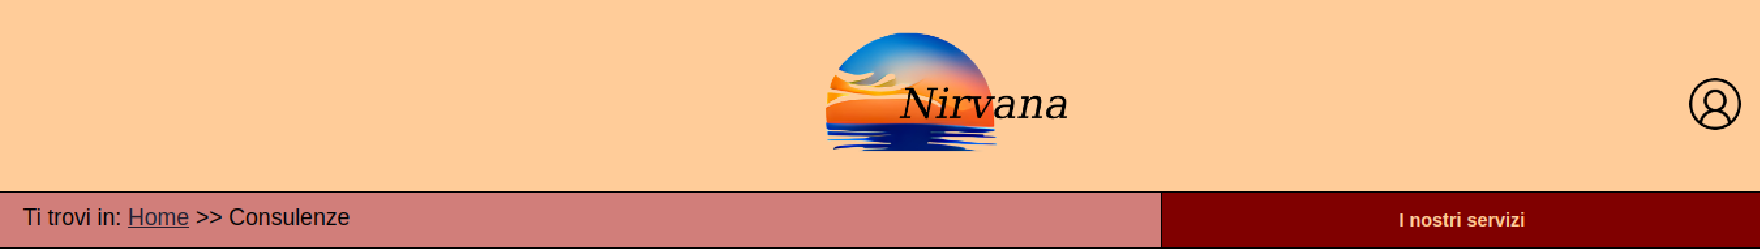
\includegraphics[width=\textwidth]{./graphics/top-common.pdf}}
	\caption{Intestazione delle pagine comprensiva di logo, breadcrumb e menù}
\end{figure}

\begin{figure}[H]
	\centering
	\fbox{
\includegraphics[width=\textwidth]{./graphics/bottom-common.pdf}}
	\caption{Footer delle pagine}
\end{figure}

In questo foglio di stile viene definita anche la struttura grafica specifica per le varie tipologie di pagine presenti nel sito:
\begin{itemize}
	\item \textbf{Pagine semplici:} sono le pagine aventi contenuti prettamente testuali (ad esempio la pagina relativa alle consulenze);
	\item \textbf{Pagine con carte:} il contenuto di tali pagine è composto da riquadri dai bordi arrotondati aventi immagini di sfondo (le "carte" appunto); i riquadri possono essere dei link ad altre pagine oppure possono contenere del testo (ad esempio per spiegare le finalità di alcuni trattamenti);
	\item \textbf{Pagine di gestione:} il contenuto di tali pagine è diviso in due metà costituite da form e/o tabelle relative alla gestione delle prenotazioni.
\end{itemize}

\begin{figure}[H]
	\centering
	\fbox{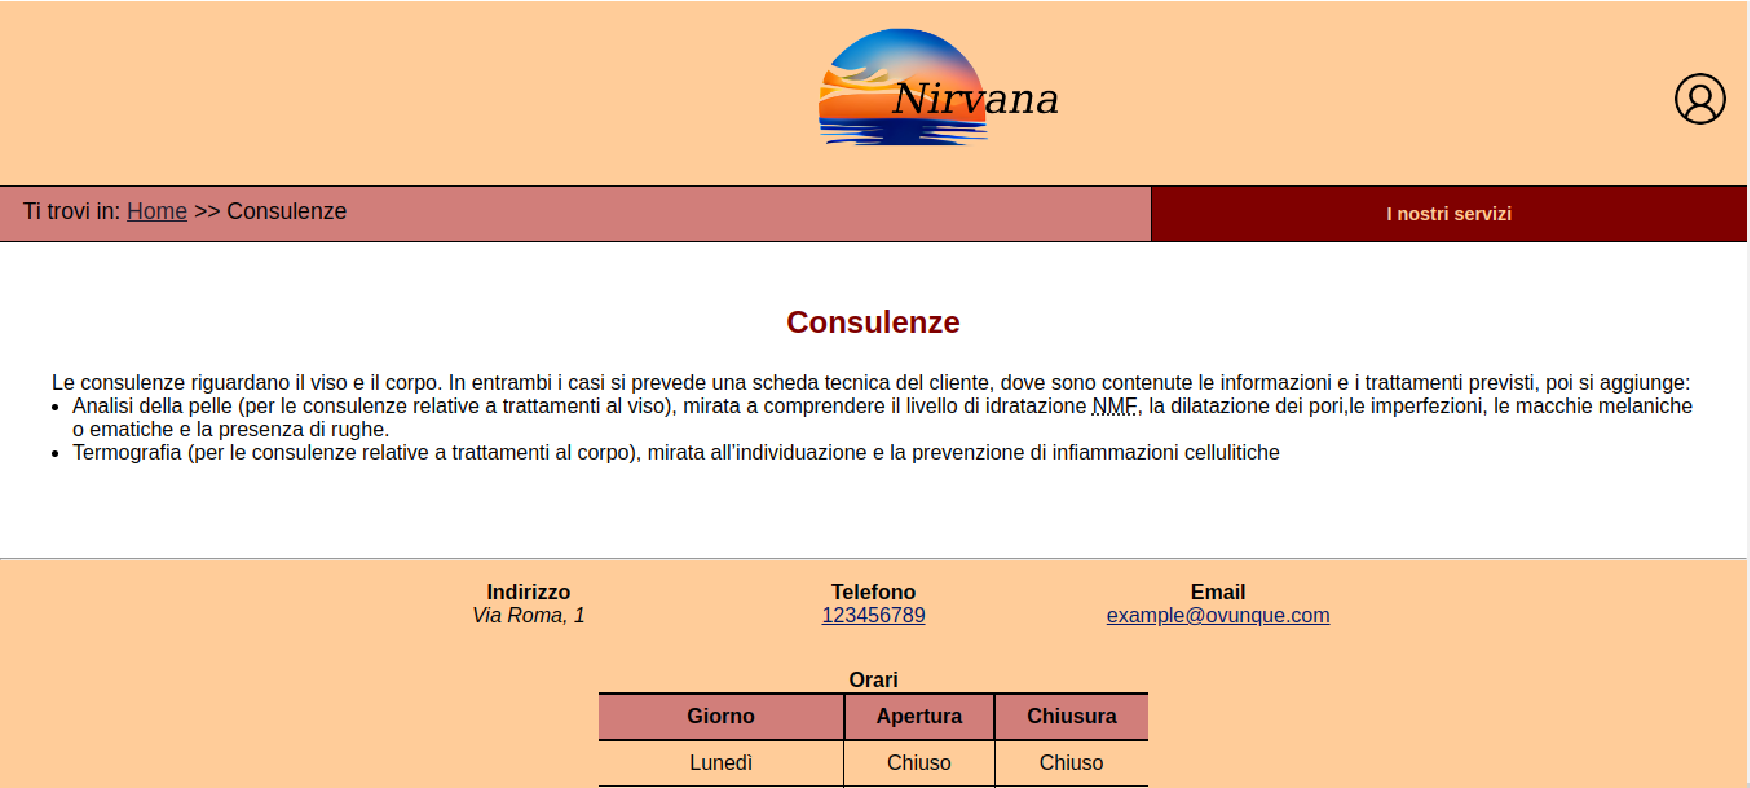
\includegraphics[width=\textwidth]{./graphics/plain-page.pdf}}
	\caption{Pagine semplici}
\end{figure}

\begin{figure}[H]
	\centering
	\fbox{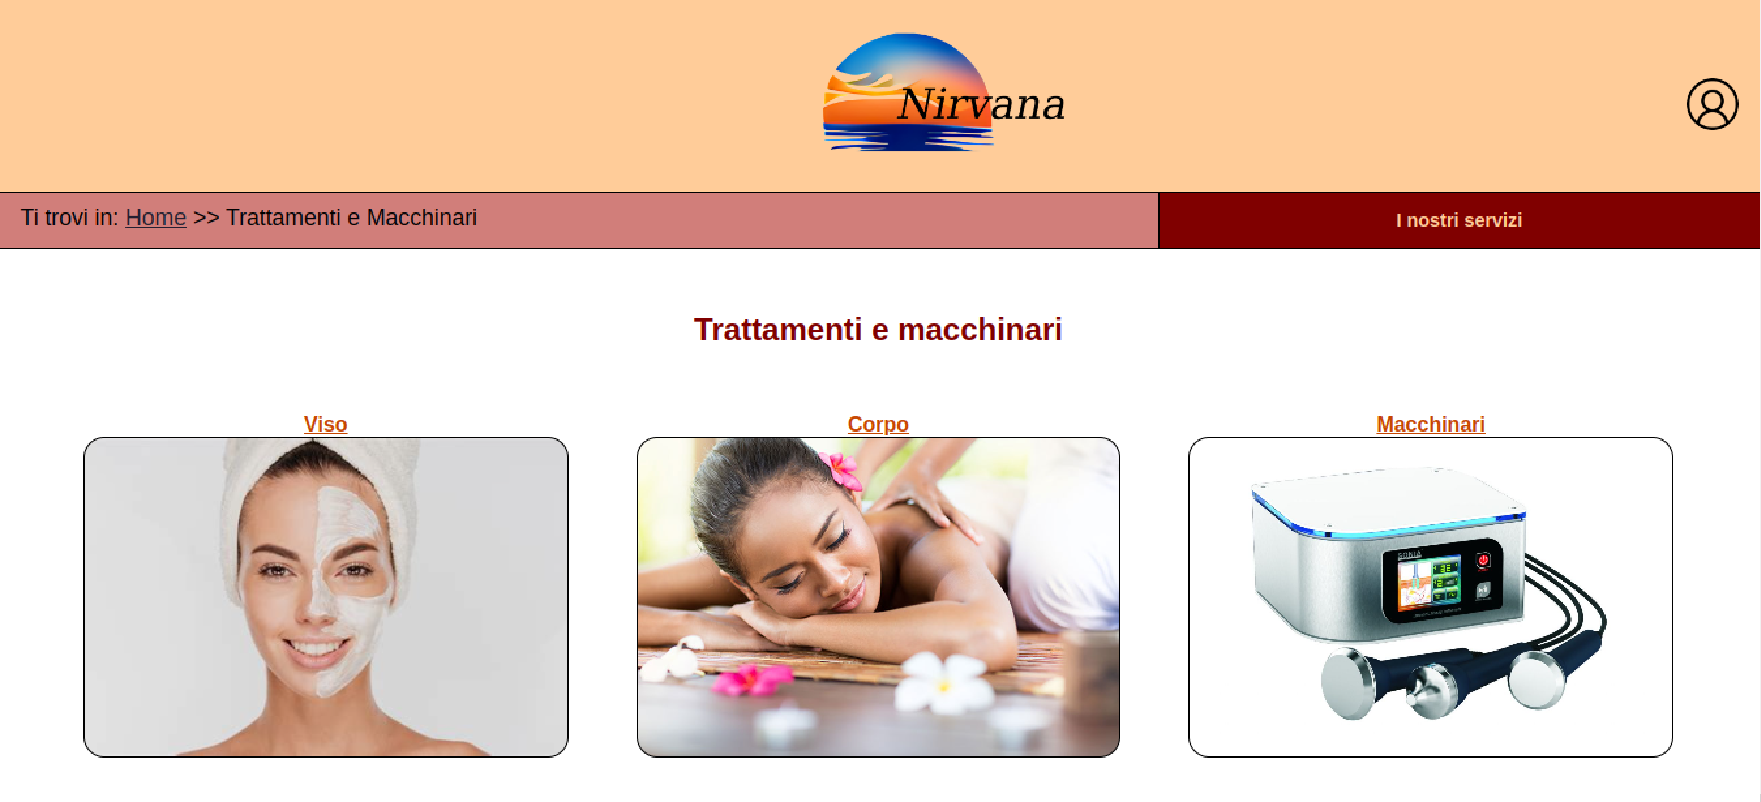
\includegraphics[width=\textwidth]{./graphics/card-page.pdf}}
	\caption{Pagine con carte}
\end{figure}

\begin{figure}[H]
	\centering
	\fbox{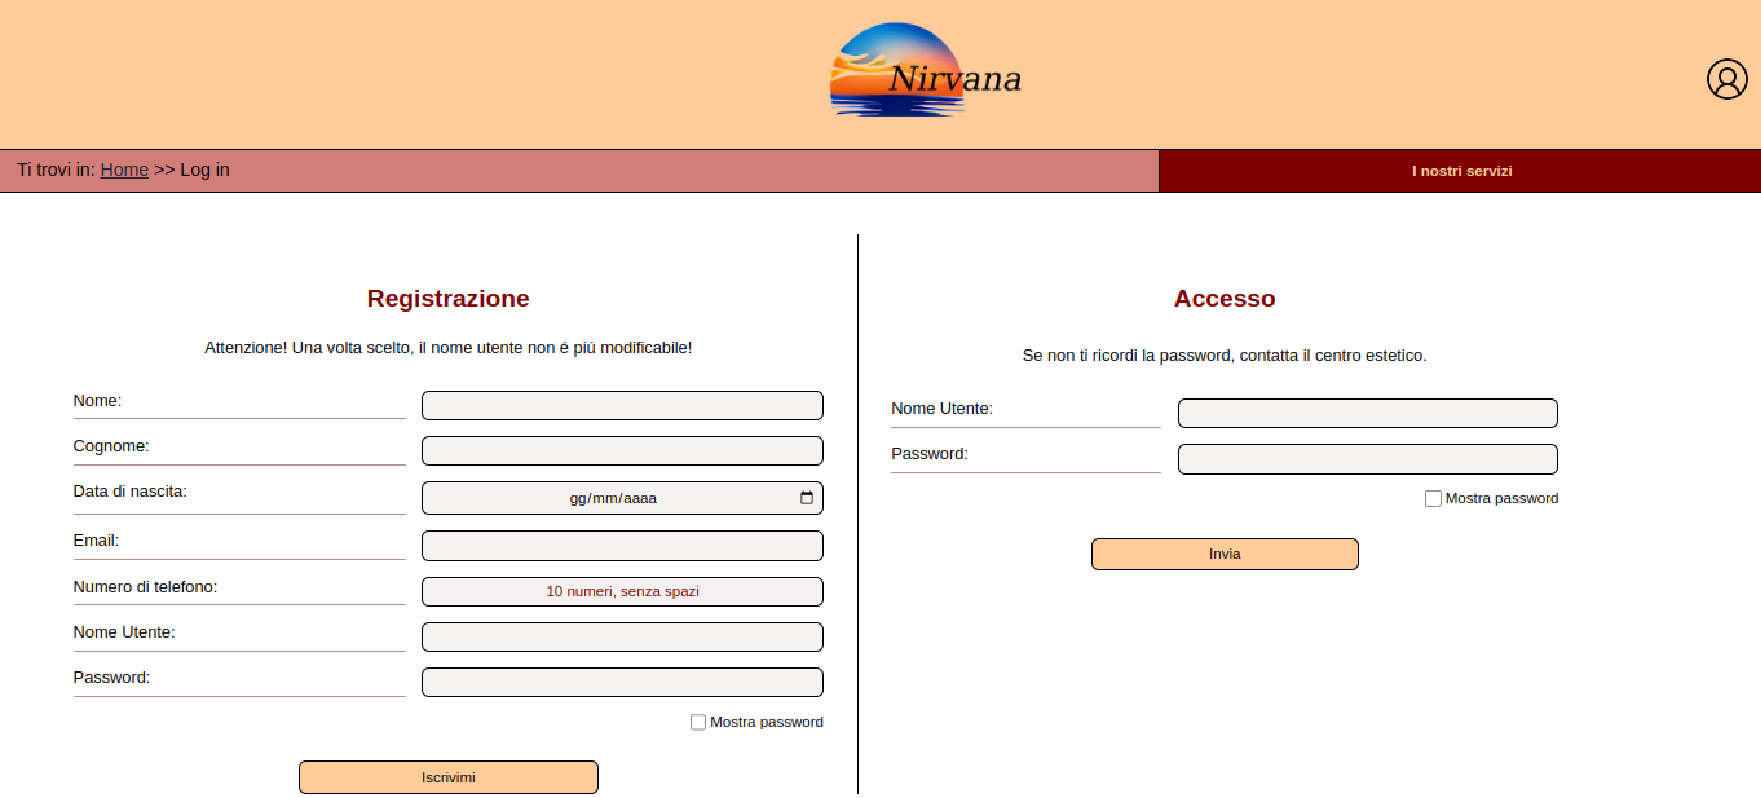
\includegraphics[width=\textwidth]{./graphics/dual-page.pdf}}
	\caption{Pagine di gestione}
\end{figure}

\subsection{Mobile}
Il foglio di stile relativo a dispositivi mobili viene utilizzato quando la larghezza di schermo offerta per la visualizzazione dei contenuti è inferiore a 1150 pixels: tale misura è stata scelta in modo sperimentale, basandosi inizialmente sulla larghezza della breadcrumb più verbosa.\\
Le principale variazioni di stile riguardano i seguenti elementi:
\begin{itemize}
	\item \textit{Tabelle:} ogni tabella viene convertita in una tabella equivalente avente una sola colonna;
	\item \textit{Grandezza carattere:} viene aumentata la grandezza dei caratteri in modo da migliorare la leggibilità;
	\item \textit{Menù:} il menù utente viene inserito sotto alla breadcrumb, offrendo le stesse funzionalità della versione desktop ma utilizzando in modo più efficiente la larghezza offerta dal dispositivo;
	\item \textit{Bottone utente:} il pulsante relativo alle azioni di login, logout ed accesso all'area personale si scorpora dall'header per rimanere fisso in una zona facilmente raggiungibile da un pollice, "appoggiandosi" sopra al footer quando si arriva a fine pagina.
\end{itemize}
Tramite \textit{media query} che si attiva quando la larghezza a disposizione per la fruizione visiva del sito è inferiore a 940 pixels, alcune breadcrumb particolamente lunghe sono sostituite da breadcrumb aventi riferimento solamente al "livello superiore", ovvero alla pagina che, nella gerarchia di navigazione del sito, si trova immediatamente sopra.
\begin{figure}[H]
	\centering
	\fbox{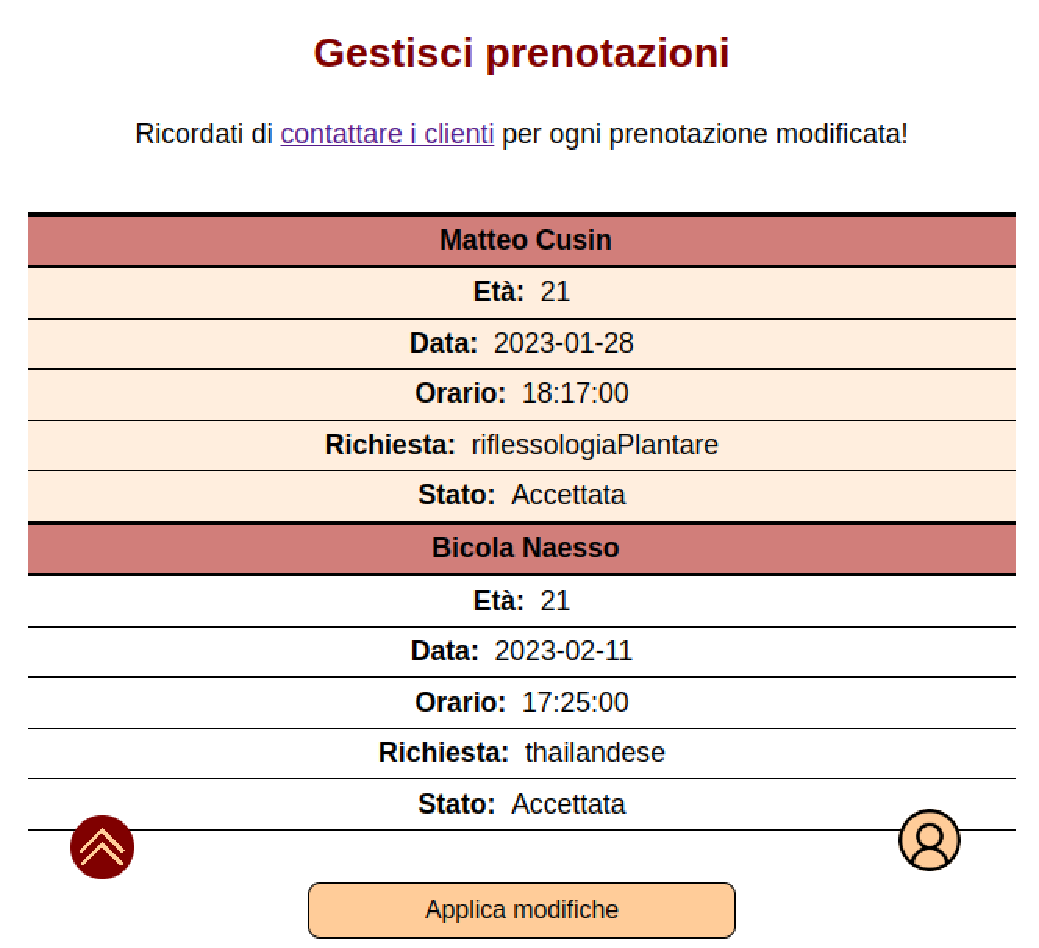
\includegraphics[height=.5\textwidth]{./graphics/table.pdf}}
	\caption{Tabella e bottone}
\end{figure}

\begin{figure}[H]
	\centering
	\fbox{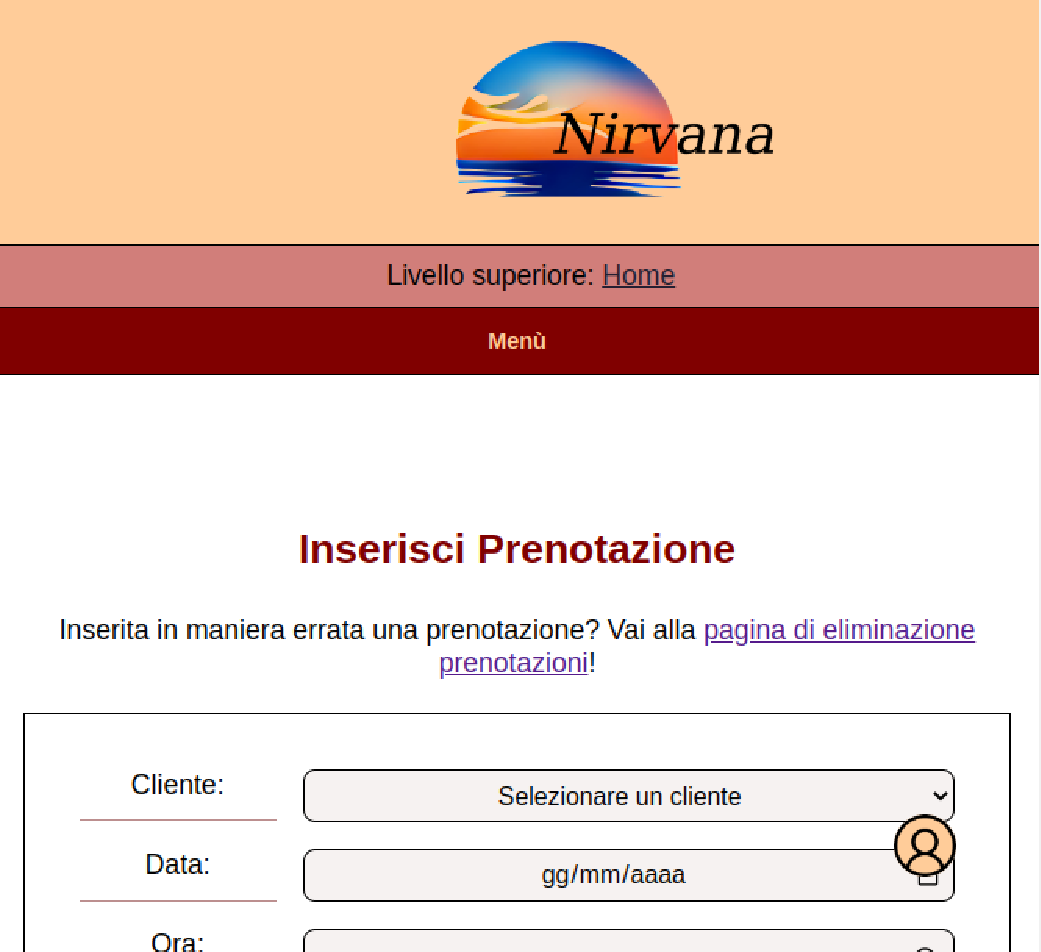
\includegraphics[height=.5\textwidth]{./graphics/menuBreadAndButton.pdf}}
	\caption{Breadcrumb, bottone e menù}
\end{figure}

%TODO Annalisa
\subsection{Wide-screen}

\subsection{Print}
Il file relativo alla stampa è stato implementato in modo tale da rimuovere le funzionalità interattive quali link, bottoni, breadcrumb e sezione menù.\\
Per facilitare la leggibilità delle informazioni in modalità cartacea, quelle che nei file .html sono classificate come carte, vengono visualizzate sottoforma di semplice testo.\\
La scelta voluta di non rimuovere il colore di background permette all'utente di scegliere l'opzione "bianco e nero" e "grafica di background" presente in ogni finestra di dialogo stampa dei motori di ricerca favorendo l'esperienza di personalizzazione.\\
Di seguito due  esempi di stampa della stessa pagina:
\begin{figure}[H]
	\centering
	\begin{subfigure}[t]{.5\textwidth}
	  \centering
	  \fbox{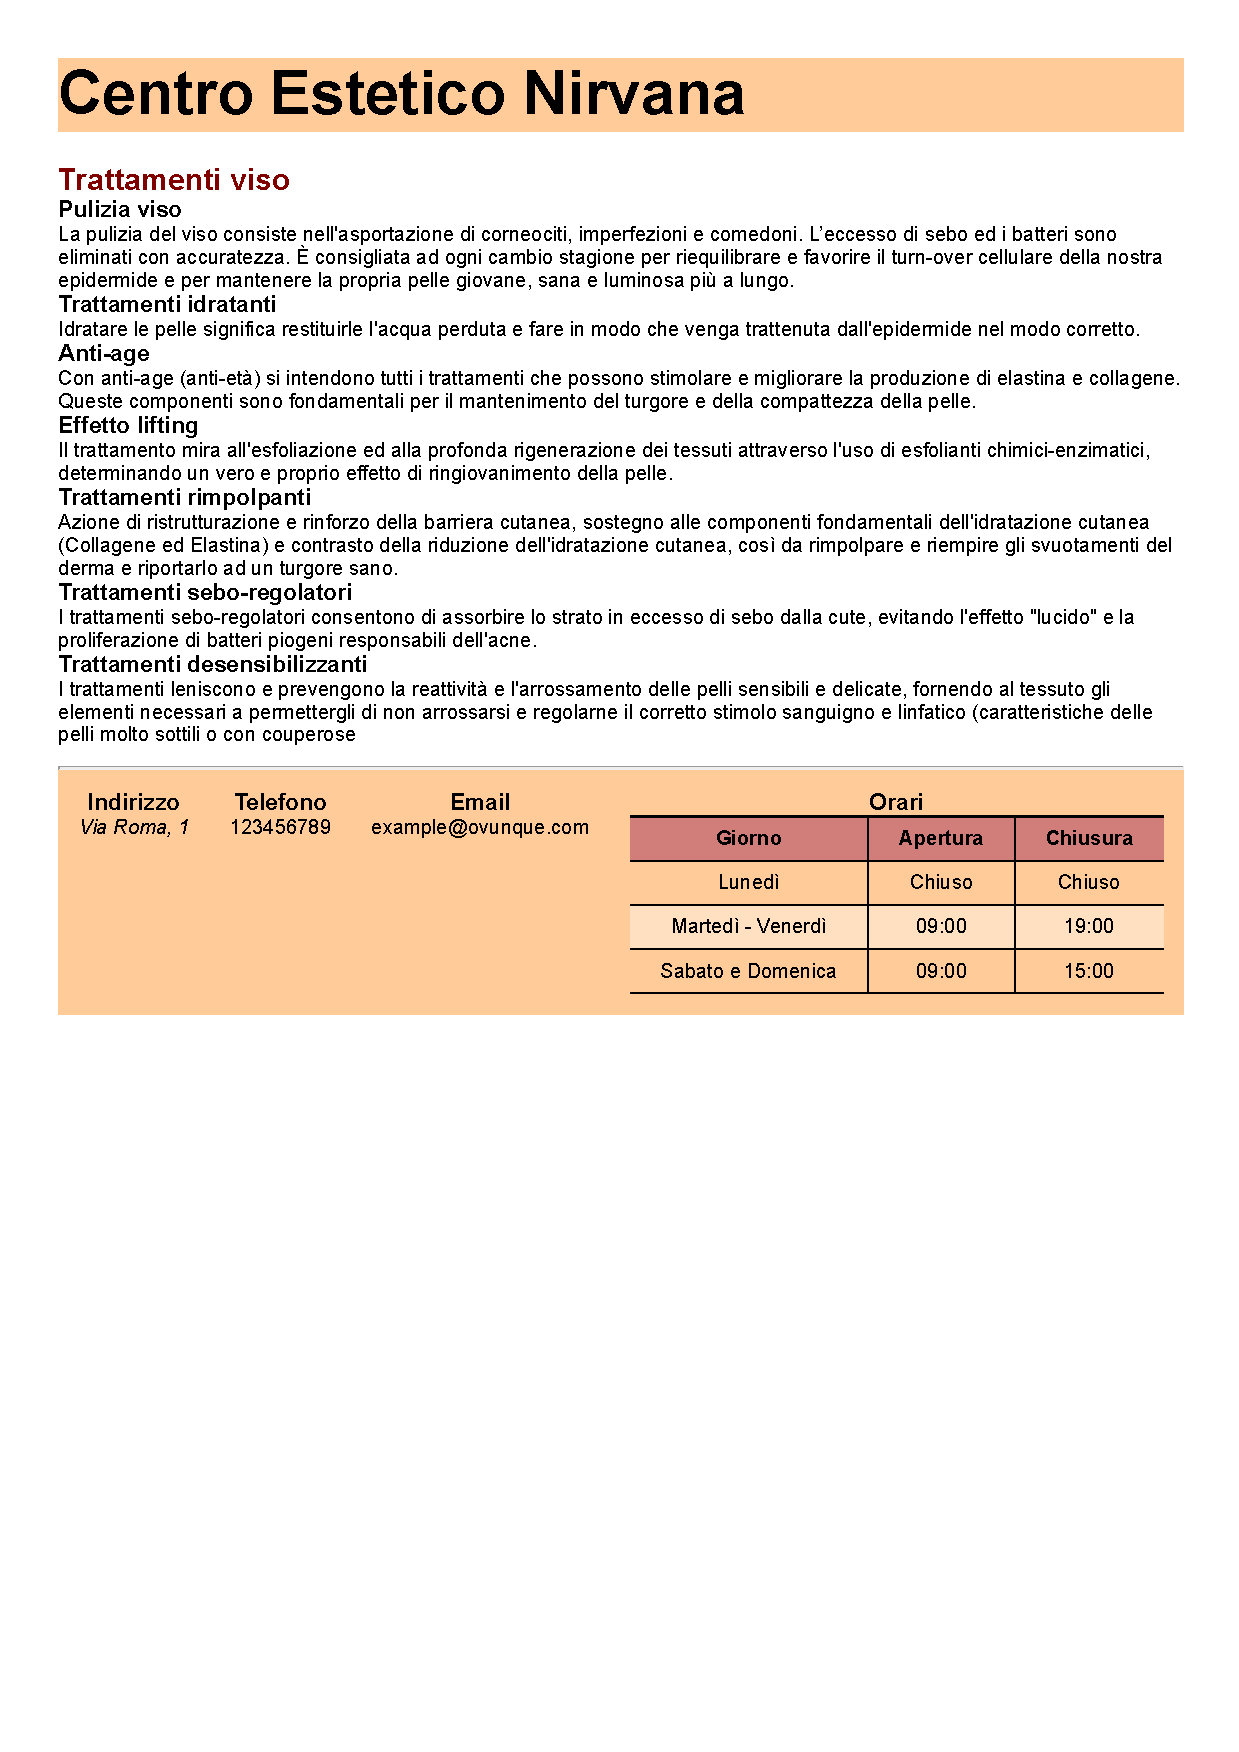
\includegraphics[width=.9\textwidth]{./graphics/NirvanaTrattamentiViso-w.pdf}}
	  \caption{Stampa con colori}
	\end{subfigure}%
	\begin{subfigure}[t]{.5\textwidth}
	  \centering
	  \fbox{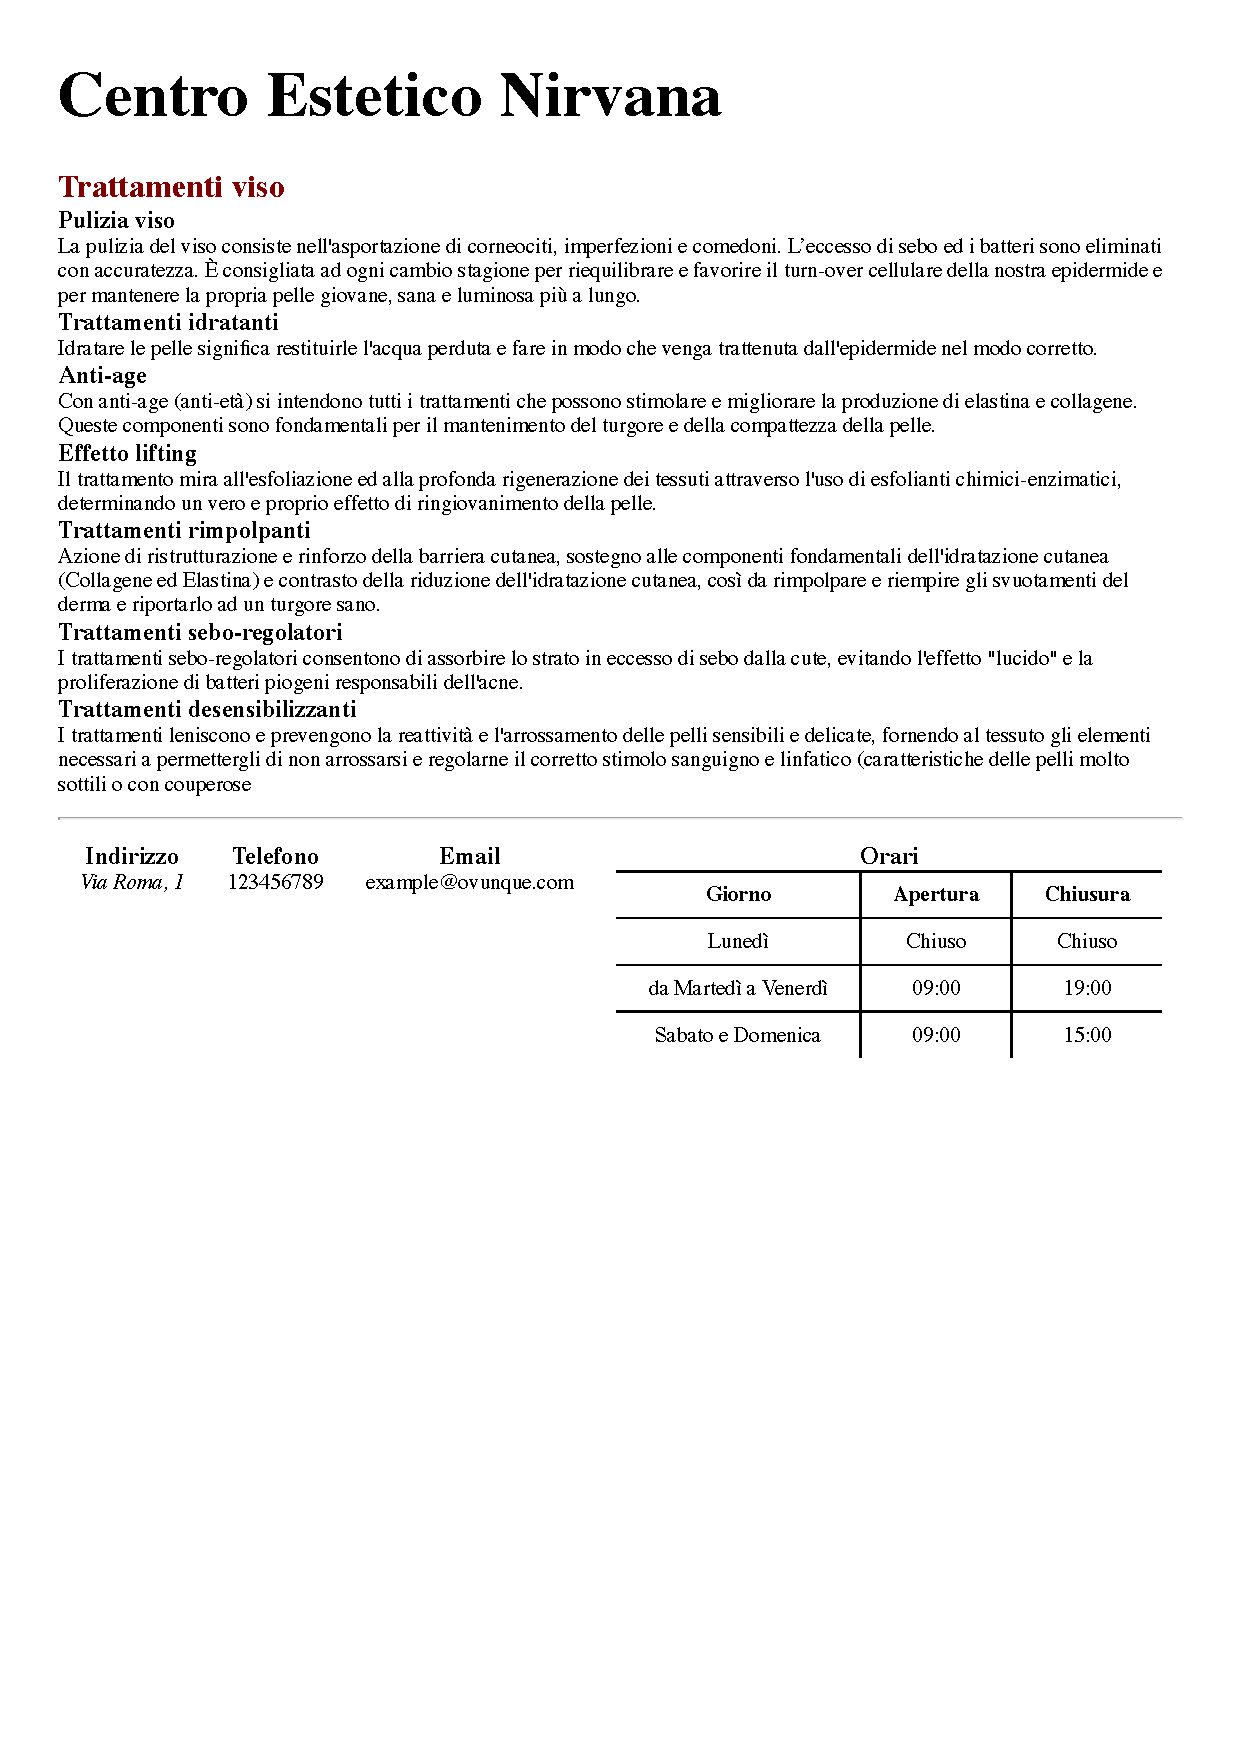
\includegraphics[width=.9\textwidth]{./graphics/NirvanaTrattamentiViso-wo.pdf}}
	  \caption{Stampa senza colori}
	\end{subfigure}
	\caption{Opzioni di stampa}
\end{figure}

%nuova sezione
\section{Implementazione}
\subsection{Linguaggi}		
\subsubsection{HTML}
Il progetto è stato realizzato tramite il linguaggio \textit{HTML5} ma si è resa possibile la compatibilità con browser più datati seguendo le linee guida del corso di Tecnologie Web e quelle del \textit{W3C}.
Si è utilizzato \textit{HTML5} piuttosto che \textit{XHTML} in quanto il pubblico cui è destinato il sito web sarà indicativamente di età compresa fra i 16 ed i 60; si presume che la clientela si distribuirà in modo omogeneo in questa fascia d'età, avente quindi a disposizione motori di ricerca tendenzialmente più recenti.\\
I file \textit{.html} si presentano con l'obbiettivo di mantenere struttura, presentazione e contenuto il più possibile separati fra loro.

Per quanto concerne i \textit{tag}:
\begin{itemize}
	\item si sono utilizzati \textit{tag} semantici che arricchiscono il progetto in accessibilità;
	\item si è controllata la chiusura di tutti i \textit{tag};
	\item i \textit{metatag} presenti nella sezione \textit{head} dei file \textit{.html} aiutano il sito nel ranking di ricerca e sono di fondamentale importanza per incrementare l'accessibilità.
\end{itemize}

\subsubsection{CSS}
La modellazione del layout del sito è stata implementata tramite CSS3.\\
Per rendere l'esperienza di navigazione fluida tra i vari dispositivi, sono state utilizzate misure relative ed in percentuale.\\
Abbiamo creato 4 fogli di stile per implementare il layout secondo lo specifico ambito d'uso:
\begin{itemize}
	\item \textit{style.css}: foglio di stile predefinito;
	\item \textit{mobile.css}: viene utilizzato dai browser nella condizione in cui lo schermo/spazio di visualizzazione abbia larghezza inferiore a 1150px;
	\item \textit{wide-screen.css}: viene utilizzato dai browser nella condizione in cui lo schermo/spazio di visualizzazione abbia larghezza superiore a 1900px;
	\item \textit{print.css}: viene presa in considerazione all'atto di stampa delle pagine del sito.
\end{itemize}
All'interno dei \textit{.css} prodotti è possibile trovare quantopiù offerto dal \textit{CSS3}, come per esempio: flexbox, grid, media queries, variabili, selettori, etc.\\
Grazie ad alcune accortezze, tramite flexbox, è stata possibile l'implementazione di un layout  "a carte" accattivante che non compromettesse l'accessibilità.

\subsection{PHP} % Matteo e Nicola
Il linguaggio PHP è stato utilizzato per lo sviluppo della parte di comportamento (server-side) del sito web.
La versione scelta dal gruppo è 8.1 dato che la 

\subsubsection{Autenticazione}
\paragraph*{Login}
\paragraph*{Logout}

\subsubsection{Connessione}

\subsubsection{Area personale}
\paragraph*{Area personale}
\paragraph*{Elenco clienti}

\subsubsection{Prenotazioni}
\paragraph*{Gestione prenotazioni lato utente}
\paragraph*{Gestione prenotazioni lato amministratore}
\paragraph*{Eliminazione prenotazioni} %Matteo

\subsubsection{Amministrazione}
\paragraph*{Errore 401}
\paragraph*{Errore 403}
\subsection{SQL}	% Nicola
\subsection{JavaScript} %Lisien
\textit{JavaScript} é un linguaggio che viene eseguito dal lato utente, quindi il browser elabora il codice. È usato per il comportamento del sito e per creare dei simulazioni nei siti.\\
Nel nostro cosa é usato per cambiare i classi di stile dei elementi HTML, e il tipo di input nei vari form e tabelle.\\
Sono i elementi che vengono modificate le classi dei stili, con l'uso di toggle, add, o remove:
\begin{itemize}
        \item \textit{Menú:} se la menú viene clicata i sui voci compaiano o spariscono a seconda del fatto di essere aperto o no. Con una semplice funzione di toggle questa viene realizato.
        \item \textit{Menú personale:} con ogni caricamento della pagina un funzione di JavaScript controlla se é stato effettuato il Log In o no. Se non é fatto allora su questa menú che compara e sparisce nel stesso modo del menú principale, viene dimostrato il link di Log In. Mentre se e stato effettuato viene dimostrato Log Out.
\end{itemize}
Con JavaScript é possibile aggiungere dei funzioni che ascoltano quando un azione e fatto dal utente. Due dei questi sono:
\begin{itemize}
        \item \textit{Click:} questa funzione semplicemente toglie le classi che fanno comparire le due menú se l'utente preme in un area che non é la menú.
        \item \textit{Scroll:} ci sono due funzioni che controllano quando l'utente fa il scroll. Uno di questi e spiegato nella sezione di sotto. L'altro controlla quando l'utente effettua il scroll per andare su. Se l'utente va su compare una pallina fissato che ti può mandare alla cima della pagina.
\end{itemize}
Altri funzioni di JavaScript sono fatti per i schermi piccoli per facilitare al utente di accedere al menú personale più facilmente. Questa funzione in particolare blocca questa menú per non andare sopra il footer della pagina.
\begin{itemize}
        \item \textit{Menú personale:} se la lunghezza della window fa superare quella della body, il funzione cambia le classi e modifica uno degli attributi, di cui é l'attributo top. Il valore del questo attributo viene calcolato dal la somma delle lunghezze della header e la body. 
\end{itemize}
L'ultima funzione che si cambia i classi e quella che fa il scroll in modalità smooth quando il bottone per andare su viene premuto.\\
Le altre funzione si occupano nel cambiamento del tipo di input:
\begin{itemize}
        \item \textit{Mostra password:} questa checkbox quando viene attivata fa cambiare il tipo di input per i password al tipo di testo
        \item \textit{Tabella admin:} su questa tabella vengono mostrate le prenotazione che devono essere accettate, rifiutate o quelle nel futuro. Se l'amministratore decide di cambiare la data o ora dei prenotazioni non accettato, il tipo di input nella tabelle viene cambiato nel formato apposto.
\end{itemize}
 
%nuova sezione
\section{Validazione}

%nuova sezione
\section{Fase di Test}

%nuova sezione
\section{Strumenti}
A supporto dello sviluppatore, é necessario che siano presenti degli strumenti per guidarlo in uno sviluppo efficiente e in un testing accurato.\\
Vengono sottolineate due categorie di strumenti poiché alcuni strumenti utilizzati non sono adatti per una fase di test, ma risultano estremamente utili come aiuto allo sviluppo.
\subsection{Strumenti di sviluppo}
\subsection{Strumenti di test}
\section{Suddivisione del lavoro}
Per garantire una buona suddivisione del carico di lavoro che il progetto ha inevitabilmente richiesto, si é suddiviso il lavoro tra i membri del gruppo in questo modo:
\begin{itemize}
	\item Lisien Skenderi: 
	\begin{itemize}
		\item HTML: Sviluppo delle seguenti pagine: Index, Consulenze, Gestione Prenotazioni - Cliente;
		\item CSS:  Elaborazione coordinata del file style.css con particolare attenzione alle sezioni header, breadcrumb e le altre navigazione
		\item Javascript: Sviluppo delle funzioni per i menú principale, menú del utente e il bottone che ti manda alla cima
		\item PHP: Backend relativo al prenotazione utente, e realizzazione della Log Out
		\item Immagini: Acquisizione usato come imagine del sfondo per i bottoni
		\item Relazione:
	\end{itemize}
	\item Matteo Cusin:
	\begin{itemize}
		\item HTML: Sviluppo delle seguenti pagine: Trattamenti Viso, Login e Registrazione, Eliminazione prenotazioni;
		\item CSS: creazione e sviluppo di mobile.css, elaborazione coordinata del file style.css con particolare attenzione alle sezioni footer e main;
		\item Javascript: funzione per mostrare in chiaro la password;
		\item PHP: backend relativo all'eliminazione delle prenotazioni;
		\item Immagini: compressione delle immagini utilizzate ed eliminazione delle immagini non utilizzate;
		\item Relazione: sezione progettazione (senza la sottosezione \textit{database}), sviluppo condiviso sezione presentazione desktop, sviluppo sezione presentazione mobile.
	\end{itemize} 
	\item Annalisa Egidi:
	\begin{itemize}
		\item HTML: Sviluppo coordinato delle seguenti pagine: 404, areaPersonale, file di trattamenti e index /**/;
		\item CSS: creazione e sviluppo di print.css, elaborazione coordinata del file style.css con particolare attenzione alle sezioni footer e main;
		\item Javascript: funzione per mostrare in chiaro la password;
		\item PHP: /**/
		\item Immagini: ricerca e modifica coordinata delle immagini, implementazione codice per l'utilizzo delle stesse;
		\item Relazione: sezione progettazione, sottosezione relativa al foglio di stile per la stampa. 
	\end{itemize} 
	\item Nicola Baesso:
	\begin{itemize}
		\item HTML: Sviluppo delle seguenti pagine: ;
		\item CSS:
		\item Javascript:
		\item PHP: backend dei form di login e registrazione, backend prenotazioni lato amministratore e cliente;
		\item Immagini:
		\item Relazione:
	\end{itemize} 
\end{itemize}

\end{document}